\chapter{移动平台设计和制造}
\label{cha:Platform}

\section{平台设计}
形式:

每个小车为一个数据点,在1-3维坐标系内动态运动(如果和ShapeBots\cite{suzuki2019shapebots}一样具备升降平台或者和SwarmOS一样具备可变色LED点阵则可以进行三维变量显示)

也可以每个小车作为一个通信节点(在电力市场的应用场景下是一个机组节点),用屏幕/位置/RGB颜色/高度直观的显示迭代的过程。

即插即用的实现:放入/取出小车,新的迭代随即开始。

\subsection{仿真}

Swarm仿真参考ShapeBots\cite{suzuki2019shapebots}的仿真方法\footnote{\href{https://ryosuzuki.github.io/shapebots-simulator/}{https://ryosuzuki.github.io/shapebots-simulator/}},使用Javascript在网页端编写了相应的仿真程序,进行指定数量的集群小车对于SVG格式图片的渲染和给定数据折线图或条形图的可视化绘制。

\subsection{定位方法}

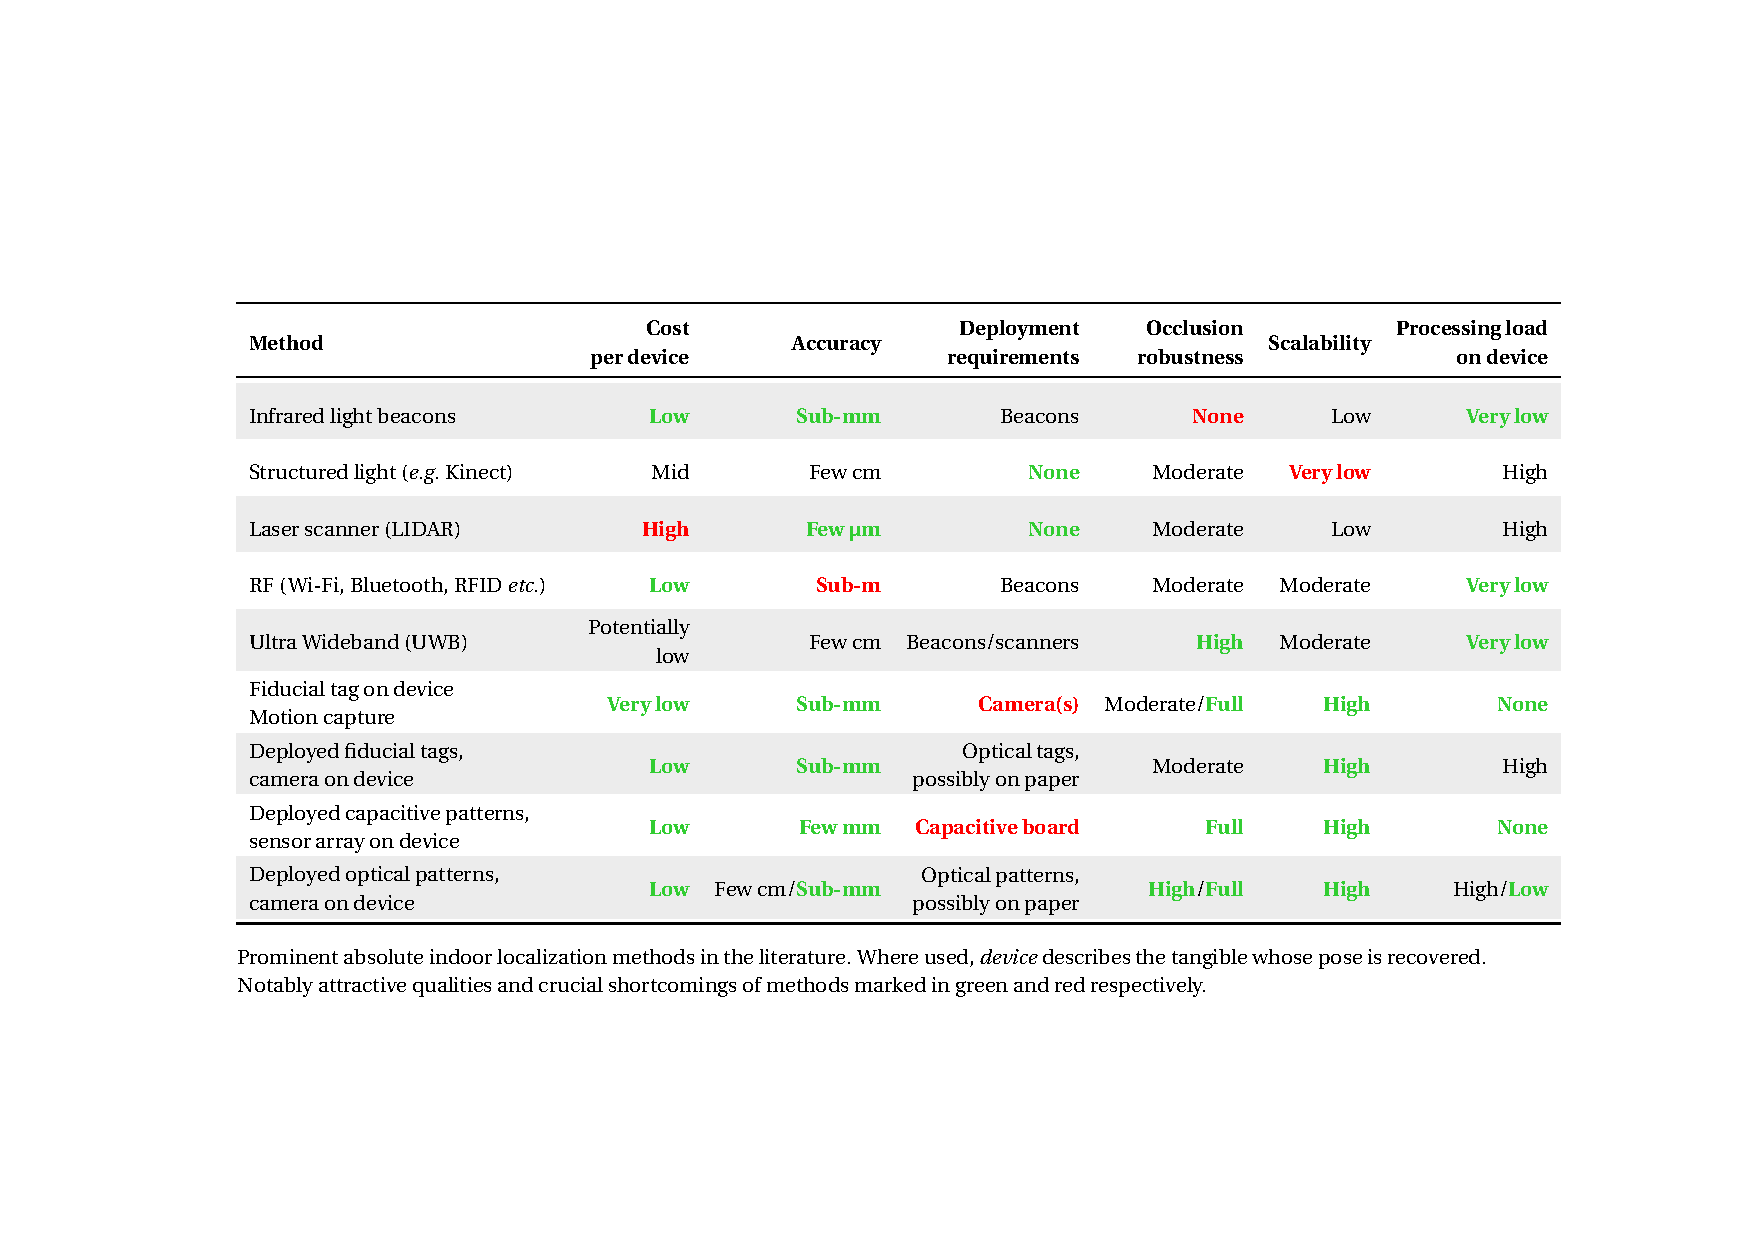
\includepdf{Prominent-absolute-indoor-localization-methods-comparison.pdf} 

各类定位方法优缺点如上述表格\cite{ozgur2018cellulo}所示。 

\subsection{底盘}
考虑到交互过程中需要推动小车,通过用户调查我们知道:大多数用户(特别是儿童)习惯于按压着移动小车,这就使得我们不能采用Zooids\cite{le2016zooids}(如图~\ref{fig:Zooids})或e-puck\cite{mondada2009puck}(如图~\ref{fig:e-puck})使用的差速转向,只能采用类似Cellulo\cite{ozgur2017cellulo}(如图~\ref{fig:Cellulo})的磁驱技术或WolfBot\cite{betthauser2014wolfbot}(如图~\ref{fig:WolfBot})使用的全向轮。

\begin{figure}[htbp]
    \centering
    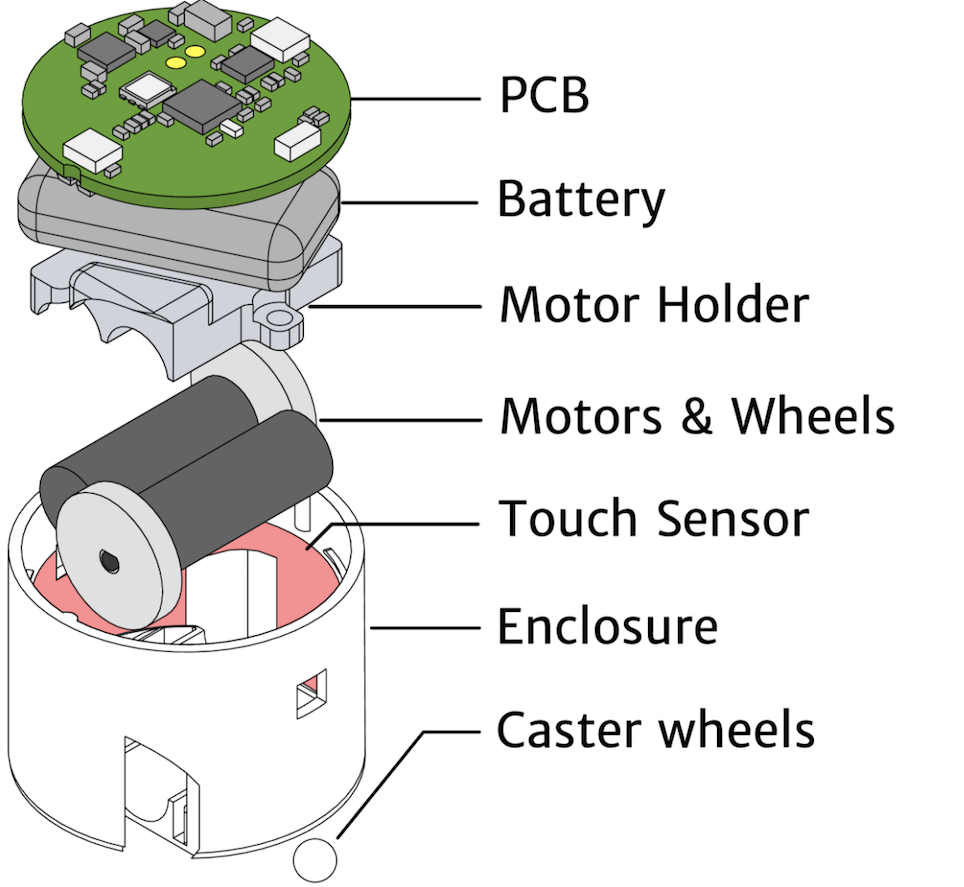
\includegraphics[height=10cm]{Zooids.png}
    \caption{Zooids}
    \label{fig:Zooids}
\end{figure}

\begin{figure}[htbp]
    \centering
    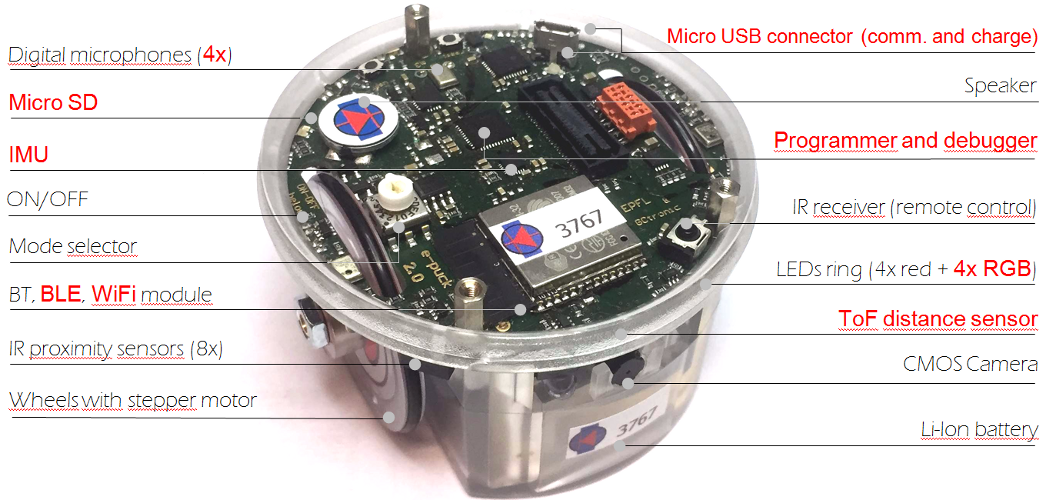
\includegraphics[height=6cm]{e-puck2-features_small.png}
    \caption{Zooids}
    \label{fig:e-puck}
\end{figure}

\begin{figure}[htbp]
    \centering
    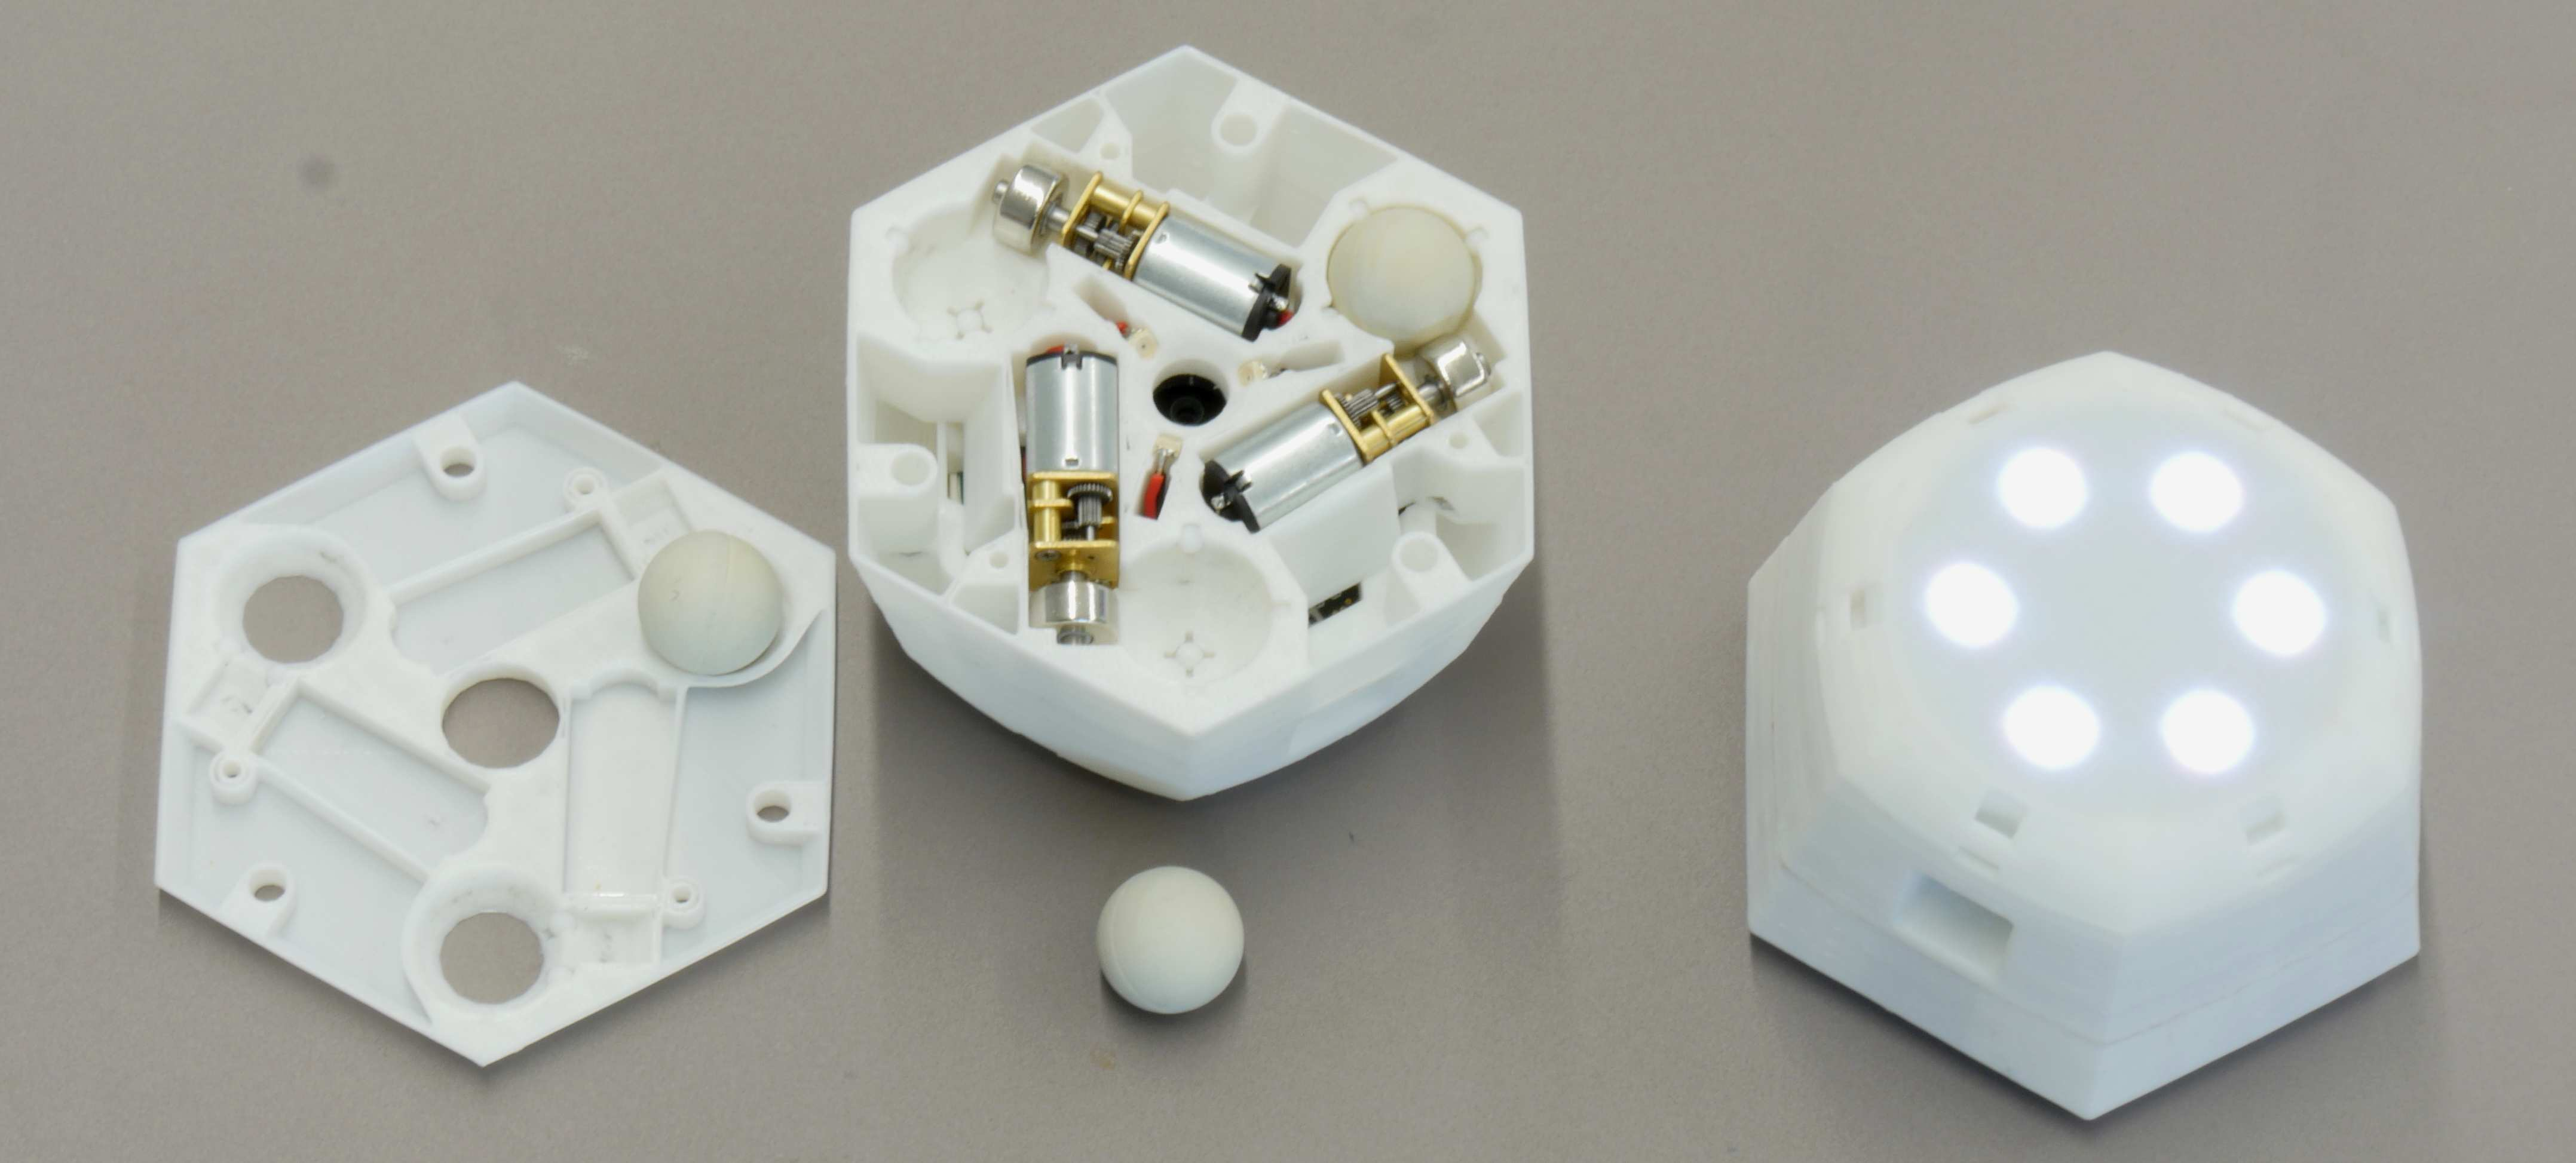
\includegraphics[height=6cm]{cellulo.jpg}
    \caption{Cellulo}
    \label{fig:Cellulo}
\end{figure}
  
\begin{figure}[htbp]
    \centering
    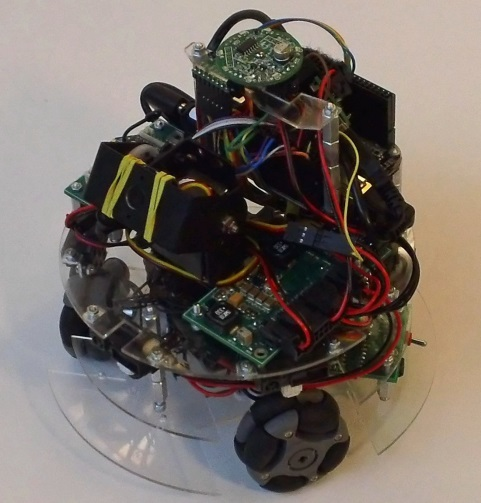
\includegraphics[height=10cm]{WolfBot.jpg}
    \caption{WolfBot}
    \label{fig:WolfBot}
\end{figure}

经过尝试,我们发现磁驱电机的速度和磁环的磁性强弱、电池的电量剩余、磁环和轴之间的胶合强度等不可控因素关系很大,无法建立起小车各轮速度和电机PWM占空比之间的时不变映射关系,导致很难控制小车的走向和速度,最终放弃了这一想法。

WolfBot采用的全向轮和电机直接连接,使得底盘占地面积很大。最终我们则采用1.5英寸麦克纳姆轮和GW12-N20减速电机(减速齿轮中的蜗杆改变90度传动方向)实现系统最小化。

\subsection{主控板}

\subsection{扩展接口}

\subsection{实物可视化界面}

\subsection{UI}